\documentclass{article}

\usepackage{tocloft}
\usepackage[utf8]{inputenc}
\usepackage[toc,page]{appendix}
\usepackage{graphicx}
\usepackage{makecell}
\usepackage{url}
\usepackage{listings}
\usepackage{caption}
\usepackage{float}
\usepackage{hyperref}

\renewcommand{\cftsecleader}{\cftdotfill{\cftdotsep}}
\renewcommand\cellgape{\Gape[4pt]}

\title{VALUE Tool Integration Manual}
\author{Vitor Freitas}
\date{May 2017}

\begin{document}

\maketitle

\begin{abstract}
This document describes to process of integrating the VALUE tool with Atlassian's JIRA and Confluence. The instructions presented herein are meant to be used with VALUE tool version 1.5 or higher. To execute all steps it is required to have administrator access on all applications, as well as access to the VALUE tool application server.
\end{abstract}

\tableofcontents

\section{JIRA}
\label{jira}
\subsection{Creating an Application User}
\label{jira_app_user}

To perform this action you will need to be signed in with a JIRA administrator user. In JIRA's administration site, open the \textbf{User management} tab and create a new user to be used by the VALUE tool.

%\begin{figure}[!t]
%    \centering
%    \noindent\makebox[\textwidth]{
%        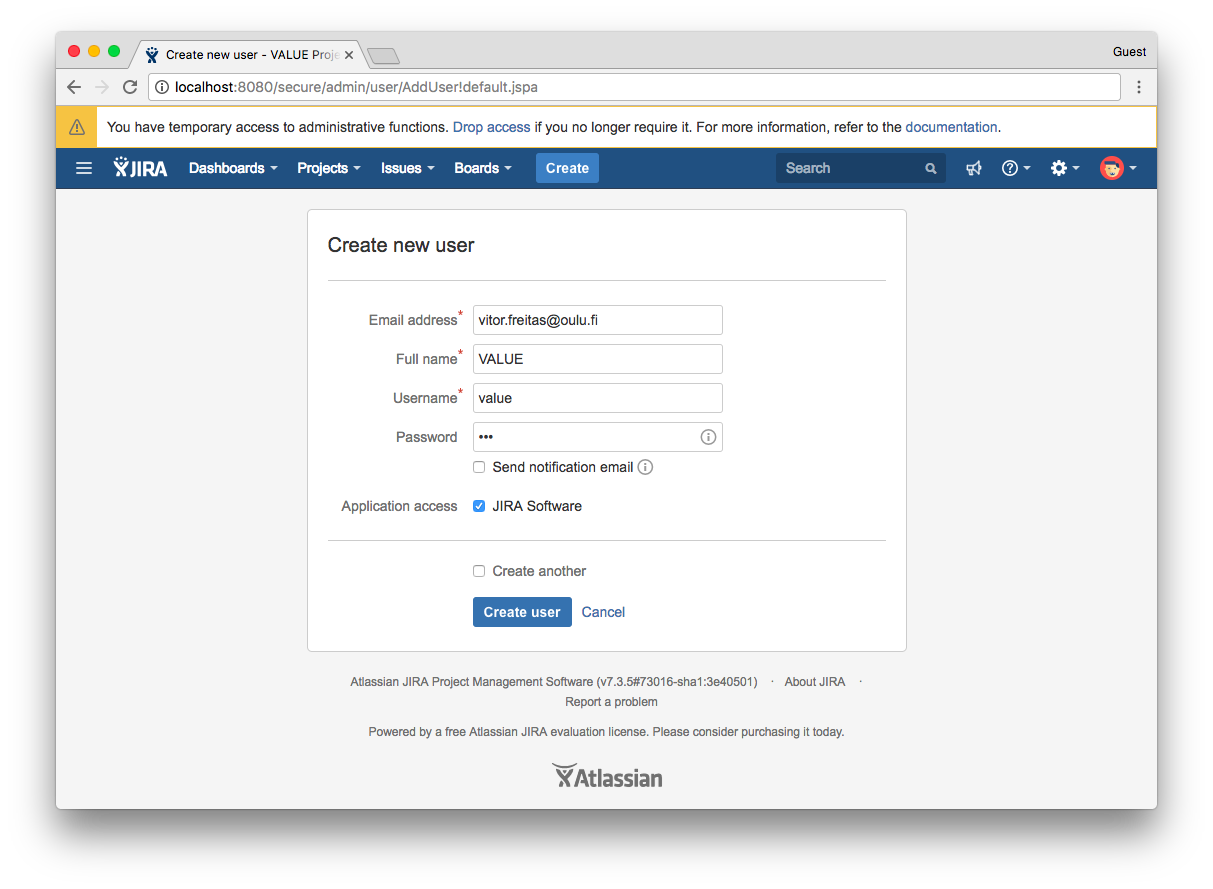
\includegraphics[width=\textwidth]{media/create_user.png}
%    }
%    \caption{Create new user}
%    \label{fig:create_user}
%\end{figure}

\subsection{Creating Custom Fields}
\label{jira_custom_fields}
Still in the JIRA's administration site, access the \textbf{Issues} tab and open the \textbf{Custom fields} screen. Create the three custom fields described in the Table \ref{tbl:custom_fields} below.

\begin{table}[!ht]
    \renewcommand{\arraystretch}{2}
    \centering
    \begin{tabular}{lll}
    \hline
    \textbf{Field name} & \textbf{Description} & \textbf{Field type}\\
    \hline
    Value Ranking & \makecell[l]{Provide the value ranking from\\the VALUE tool} & Number Field\\
    
    Value Summary & \makecell[l]{Provide the group assessment\\summary from the VALUE tool} & Text Field (multi-line)\\
    
    Value URL & \makecell[l]{URL of the issue on the\\VALUE tool} & URL Field\\
    \hline
    \end{tabular}
    \caption{Custom fields}
    \label{tbl:custom_fields}
\end{table}

In the \textbf{Issues} tab, access the \textbf{Field configurations} and click on \textbf{configure}. Set the renderer of the \textbf{Value Summary} field to \textbf{Wiki Style Renderer}.

%\begin{figure}[!t]
%    \centering
%    \noindent\makebox[\textwidth]{
%        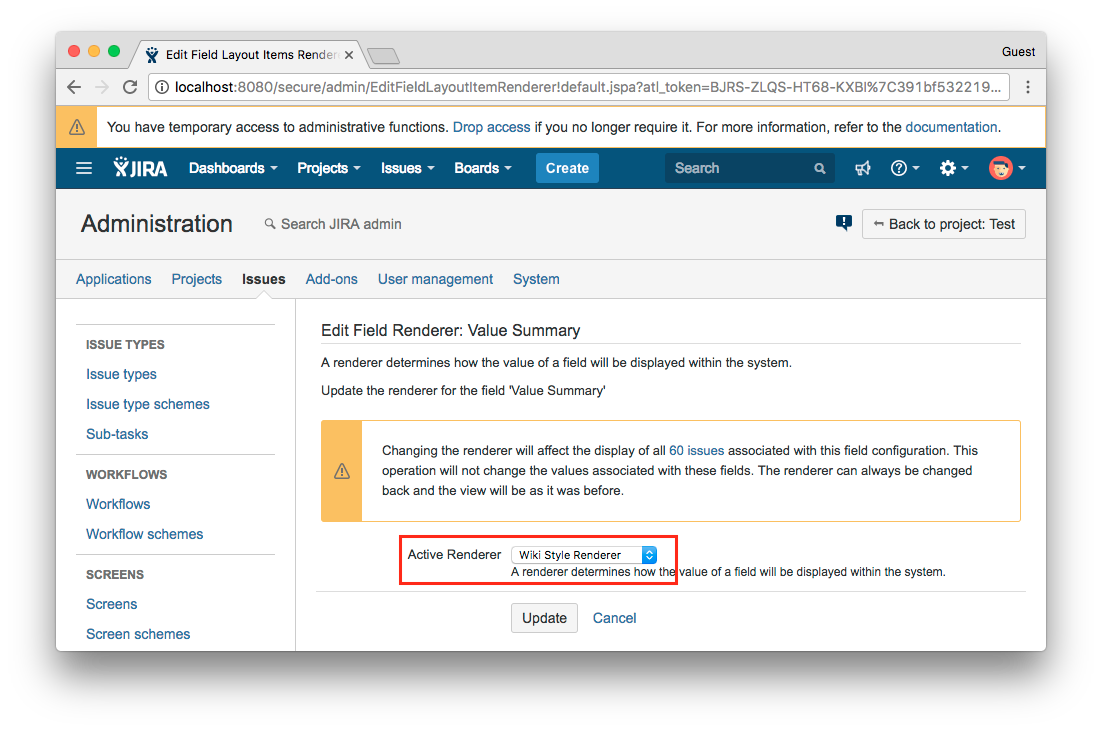
\includegraphics[width=\textwidth]{media/value_summary_renderer.png}
%    }
%    \caption{Edit Field Renderer: Value Summary}
%    \label{fig:value_summary_renderer}
%\end{figure}

\section{VALUE Tool}
\label{value}
\subsection{Connecting with JIRA's REST API}
To perform this task you will need access to the application server where the VALUE tool is deployed.

Edit the \textbf{.env} file located in the project root (\url{/opt/value_tool/value/.env}). Add the following environment variables accordingly to Figure \ref{fig:value_env}.

\begin{itemize}
    \item \texttt{JIRA\_URL}: base URL of the JIRA installation
    \item \texttt{JIRA\_USERNAME}: username defined in Section \ref{jira_app_user}
    \item \texttt{JIRA\_PASSWORD}: password defined in Section \ref{jira_app_user}
\end{itemize}

\begin{figure}[!t]
    \centering
    \noindent\makebox[\textwidth]{
        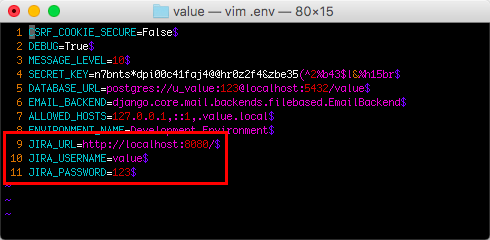
\includegraphics[width=\textwidth]{media/value_env.png}
    }
    \caption{JIRA credentials}
    \label{fig:value_env}
\end{figure}

\subsection{Mapping JIRA's Custom Fields}
In the VALUE tool, open the \textbf{Application settings} screen and click on the \textbf{JIRA integration} menu. Check the \textbf{Enable JIRA integration} option and inform the IDs of the JIRA custom fields created in Section \ref{jira_custom_fields} (see Figure \ref{fig:value_jira}).

\begin{figure}[!t]
    \centering
    \noindent\makebox[\textwidth]{
        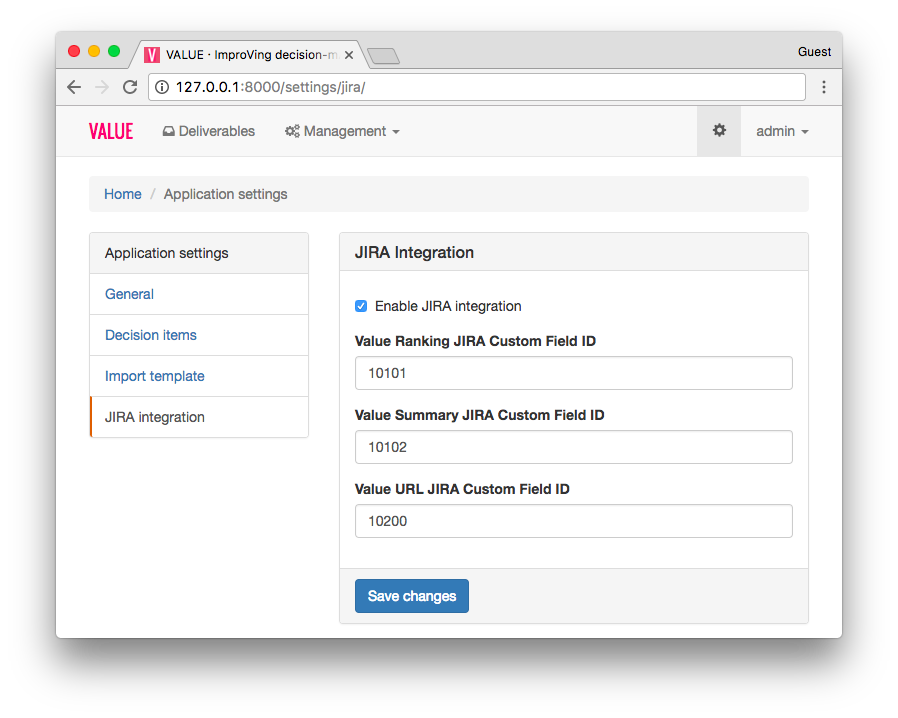
\includegraphics[width=\textwidth]{media/value_jira.png}
    }
    \caption{VALUE tool JIRA configuration}
    \label{fig:value_jira}
\end{figure}

\section{Confluence}
\label{confluence}

To install the \textbf{User Macros} properly, download the templates in plain text using the link: \url{http://valueproject.fi/macros/}

\subsection{Creating User Macros}
Inside the \textbf{Confluence administration}, access the \textbf{User Macros} screen to create the following macros described below.

\subsubsection{Value Charts Macro}

\begin{itemize}
    \item \textbf{Macro Name:} value\_charts
    \item \textbf{Macro Title:} Value Charts
    \item \textbf{Description:} Renders a chart from the VALUE tool's dashboard
    \item \textbf{Categories:} Development
    \item \textbf{Macro Body Processing:} No macro body
\end{itemize}

\textbf{Template:}

\begin{lstlisting}[frame=single]
## Macro title: Value Charts
## Macro has a body: N
##
## Developed by: Vitor Freitas
## Date created: 05/05/2017
## Installed by: <INSTALLER_NAME>

## @param ChartType:title=Chart Type|type=enum|
enumValues=decision_items_overview,value_ranking,
factors_comparison|default=red|desc=Choose a chart type
## @param IssueId:title=Issue ID|type=string|
desc=JIRA Issue ID
## @param Width:title=Width|type=string|default=500|
desc=Width of the chart
## @param Height:title=Height|type=string|default=400|
desc=Height of the chart

<iframe style="border:0;padding:0;margin:0;" 
width="$paramWidth" height="$paramHeight" 
src="https://<VALUE_TOOL_DOMAIN>/api/charts/
?id=$paramIssueId&chartType=$paramChartType"></iframe>
\end{lstlisting}

Change the \texttt{\textless INSTALLER\_NAME\textgreater} and \texttt{\textless VALUE\_TOOL\_DOMAIN\textgreater} markups with the correct values.

\subsubsection{Value Summary Macro}

\begin{itemize}
    \item \textbf{Macro Name:} value\_summary
    \item \textbf{Macro Title:} Value Summary
    \item \textbf{Description:} Display the evaluation summary from the VALUE tool
    \item \textbf{Categories:} Development
    \item \textbf{Macro Body Processing:} No macro body
\end{itemize}

\textbf{Template:}

\begin{lstlisting}[frame=single]
## Macro title: Value Summary
## Macro has a body: N
##
## Developed by: Vitor Freitas
## Date created: 05/05/2017
## Installed by: <INSTALLER_NAME>

## This is an example macro
## @param IssueId:title=IssueId|type=string|
required=true|desc=JIRA Issue ID

<iframe style="border:0;padding:0;margin:0;" width="100%" 
height="20" src="https://<VALUE_TOOL_DOMAIN>/api/summary/
?id=$paramIssueId"></iframe>

\end{lstlisting}

Change the \texttt{\textless INSTALLER\_NAME\textgreater} and \texttt{\textless VALUE\_TOOL\_DOMAIN\textgreater} markups with the correct values.

\begin{appendices}
\section{JIRA Integration Screenshots}

\begin{figure}[H]
    \centering
    \captionsetup{labelformat=empty}
    \caption{Import issues from JIRA directly in the VALUE tool}
    \noindent\makebox[\textwidth]{
        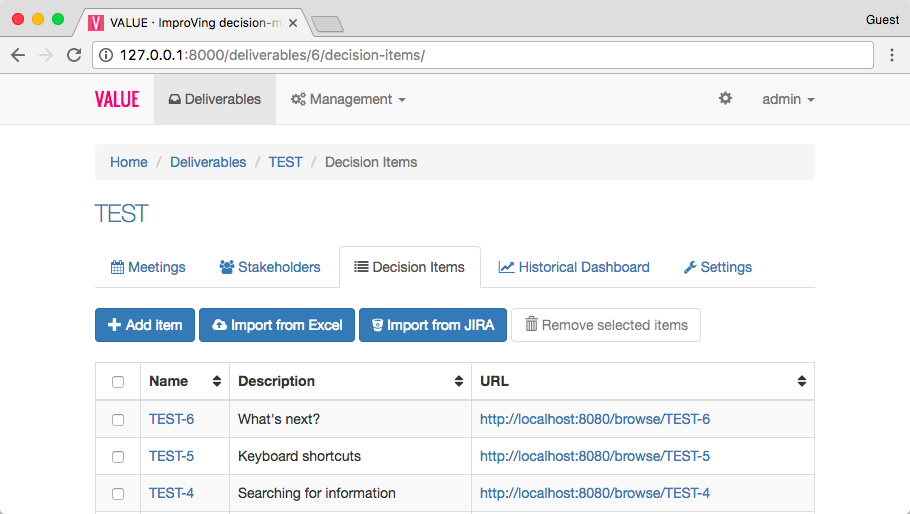
\includegraphics[width=\textwidth]{media/appendix_1.png}
    }
\end{figure}

\begin{figure}[H]
    \centering
    \captionsetup{labelformat=empty}
    \caption{Select the issues to import}
    \noindent\makebox[\textwidth]{
        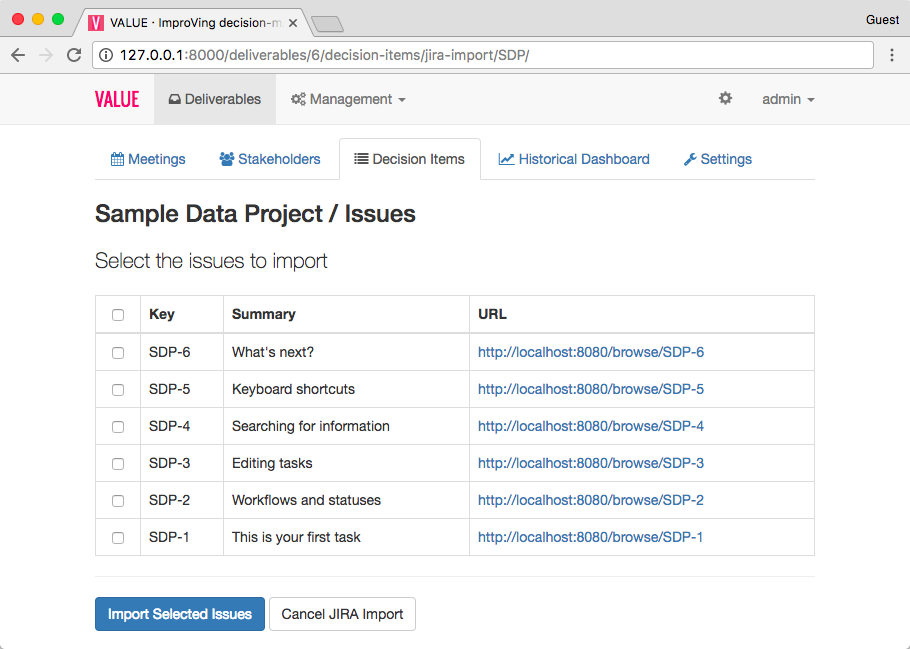
\includegraphics[width=\textwidth]{media/appendix_2.png}
    }
\end{figure}

\begin{figure}[H]
    \centering
    \captionsetup{labelformat=empty}
    \caption{Sync the data back to JIRA}
    \noindent\makebox[\textwidth]{
        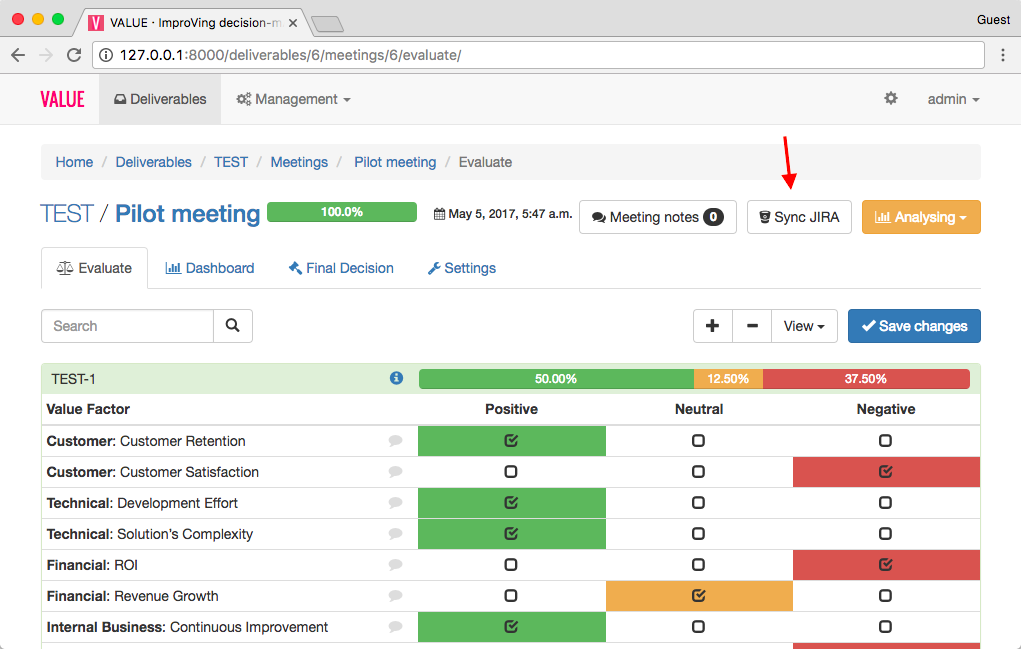
\includegraphics[width=\textwidth]{media/appendix_3.png}
    }
\end{figure}

\begin{figure}[H]
    \centering
    \captionsetup{labelformat=empty}
    \caption{Visualize the value of the issues/features in JIRA}
    \noindent\makebox[\textwidth]{
        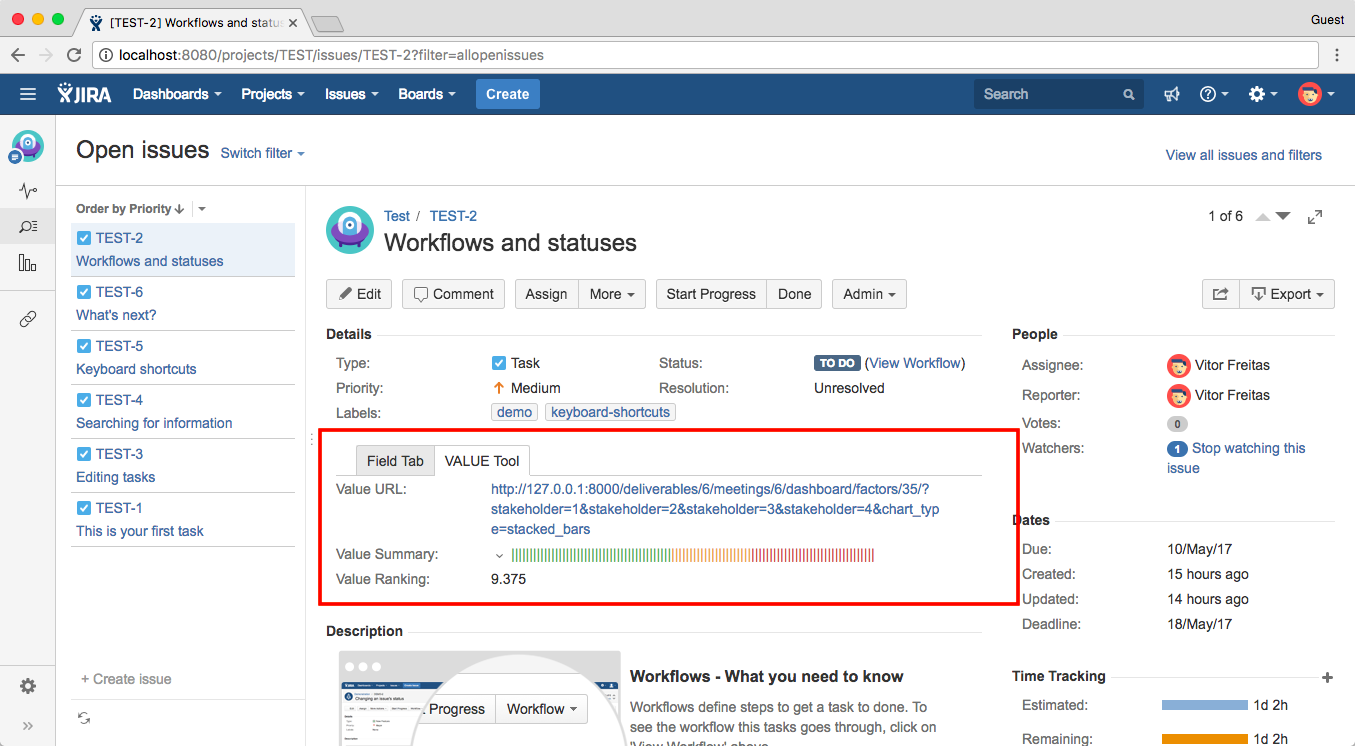
\includegraphics[width=\textwidth]{media/appendix_4.png}
    }
\end{figure}

\begin{figure}[H]
    \centering
    \captionsetup{labelformat=empty}
    \caption{Display the value data in Confluence pages}
    \noindent\makebox[\textwidth]{
        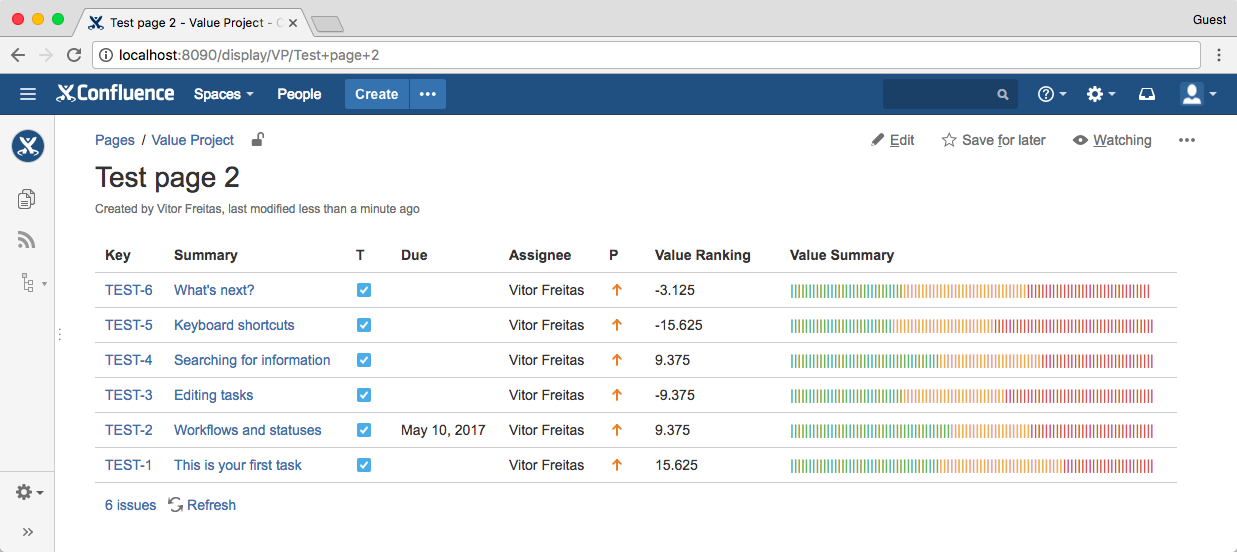
\includegraphics[width=\textwidth]{media/appendix_5.png}
    }
\end{figure}

\begin{figure}[H]
    \centering
    \captionsetup{labelformat=empty}
    \caption{Use custom user macros on Confluence}
    \noindent\makebox[\textwidth]{
        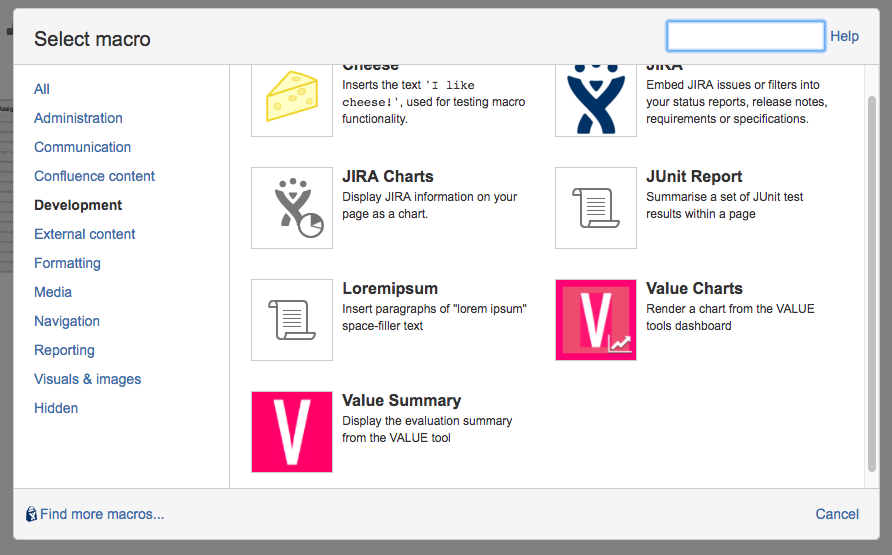
\includegraphics[width=\textwidth]{media/appendix_7.png}
    }
\end{figure}

\begin{figure}[H]
    \centering
    \captionsetup{labelformat=empty}
    \caption{Use value charts embedded to Confluence pages}
    \noindent\makebox[\textwidth]{
        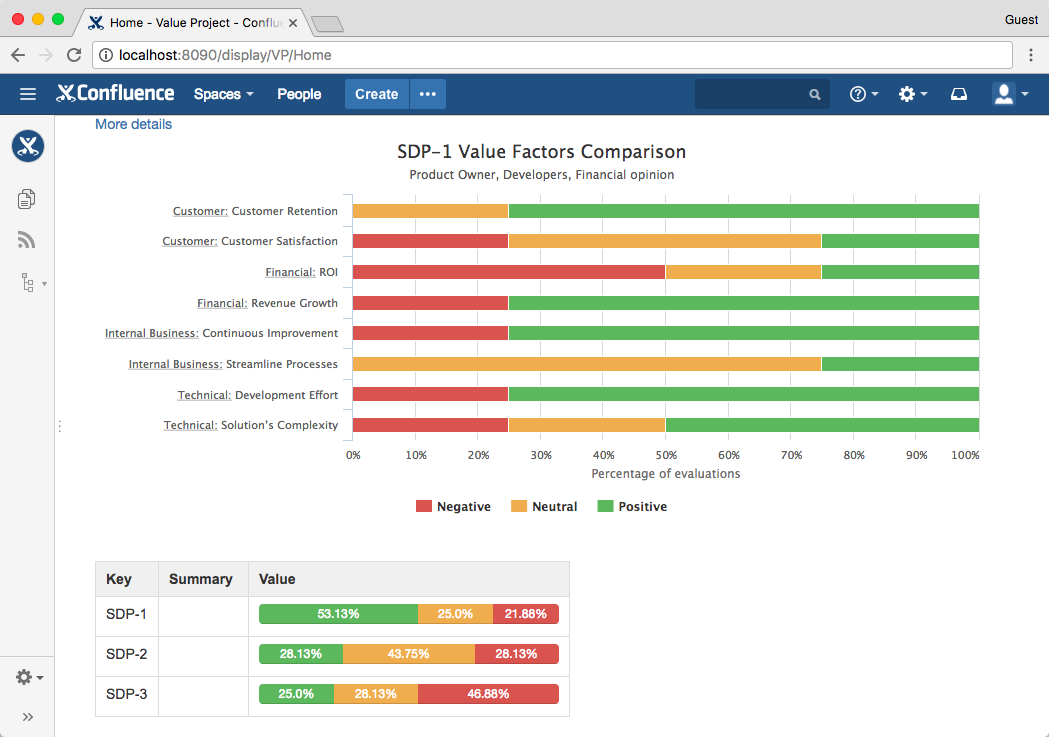
\includegraphics[width=\textwidth]{media/appendix_6.png}
    }
\end{figure}

\end{appendices}

\end{document}
